\documentclass[1p]{elsarticle_modified}
%\bibliographystyle{elsarticle-num}

%\usepackage[colorlinks]{hyperref}
%\usepackage{abbrmath_seonhwa} %\Abb, \Ascr, \Acal ,\Abf, \Afrak
\usepackage{amsfonts}
\usepackage{amssymb}
\usepackage{amsmath}
\usepackage{amsthm}
\usepackage{scalefnt}
\usepackage{amsbsy}
\usepackage{kotex}
\usepackage{caption}
\usepackage{subfig}
\usepackage{color}
\usepackage{graphicx}
\usepackage{xcolor} %% white, black, red, green, blue, cyan, magenta, yellow
\usepackage{float}
\usepackage{setspace}
\usepackage{hyperref}

\usepackage{tikz}
\usetikzlibrary{arrows}

\usepackage{multirow}
\usepackage{array} % fixed length table
\usepackage{hhline}

%%%%%%%%%%%%%%%%%%%%%
\makeatletter
\renewcommand*\env@matrix[1][\arraystretch]{%
	\edef\arraystretch{#1}%
	\hskip -\arraycolsep
	\let\@ifnextchar\new@ifnextchar
	\array{*\c@MaxMatrixCols c}}
\makeatother %https://tex.stackexchange.com/questions/14071/how-can-i-increase-the-line-spacing-in-a-matrix
%%%%%%%%%%%%%%%

\usepackage[normalem]{ulem}

\newcommand{\msout}[1]{\ifmmode\text{\sout{\ensuremath{#1}}}\else\sout{#1}\fi}
%SOURCE: \msout is \stkout macro in https://tex.stackexchange.com/questions/20609/strikeout-in-math-mode

\newcommand{\cancel}[1]{
	\ifmmode
	{\color{red}\msout{#1}}
	\else
	{\color{red}\sout{#1}}
	\fi
}

\newcommand{\add}[1]{
	{\color{blue}\uwave{#1}}
}

\newcommand{\replace}[2]{
	\ifmmode
	{\color{red}\msout{#1}}{\color{blue}\uwave{#2}}
	\else
	{\color{red}\sout{#1}}{\color{blue}\uwave{#2}}
	\fi
}

\newcommand{\Sol}{\mathcal{S}} %segment
\newcommand{\D}{D} %diagram
\newcommand{\A}{\mathcal{A}} %arc


%%%%%%%%%%%%%%%%%%%%%%%%%%%%%5 test

\def\sl{\operatorname{\textup{SL}}(2,\Cbb)}
\def\psl{\operatorname{\textup{PSL}}(2,\Cbb)}
\def\quan{\mkern 1mu \triangleright \mkern 1mu}

\theoremstyle{definition}
\newtheorem{thm}{Theorem}[section]
\newtheorem{prop}[thm]{Proposition}
\newtheorem{lem}[thm]{Lemma}
\newtheorem{ques}[thm]{Question}
\newtheorem{cor}[thm]{Corollary}
\newtheorem{defn}[thm]{Definition}
\newtheorem{exam}[thm]{Example}
\newtheorem{rmk}[thm]{Remark}
\newtheorem{alg}[thm]{Algorithm}

\newcommand{\I}{\sqrt{-1}}
\begin{document}

%\begin{frontmatter}
%
%\title{Boundary parabolic representations of knots up to 8 crossings}
%
%%% Group authors per affiliation:
%\author{Yunhi Cho} 
%\address{Department of Mathematics, University of Seoul, Seoul, Korea}
%\ead{yhcho@uos.ac.kr}
%
%
%\author{Seonhwa Kim} %\fnref{s_kim}}
%\address{Center for Geometry and Physics, Institute for Basic Science, Pohang, 37673, Korea}
%\ead{ryeona17@ibs.re.kr}
%
%\author{Hyuk Kim}
%\address{Department of Mathematical Sciences, Seoul National University, Seoul 08826, Korea}
%\ead{hyukkim@snu.ac.kr}
%
%\author{Seokbeom Yoon}
%\address{Department of Mathematical Sciences, Seoul National University, Seoul, 08826,  Korea}
%\ead{sbyoon15@snu.ac.kr}
%
%\begin{abstract}
%We find all boundary parabolic representation of knots up to 8 crossings.
%
%\end{abstract}
%\begin{keyword}
%    \MSC[2010] 57M25 
%\end{keyword}
%
%\end{frontmatter}

%\linenumbers
%\tableofcontents
%
\newcommand\colored[1]{\textcolor{white}{\rule[-0.35ex]{0.8em}{1.4ex}}\kern-0.8em\color{red} #1}%
%\newcommand\colored[1]{\textcolor{white}{ #1}\kern-2.17ex	\textcolor{white}{ #1}\kern-1.81ex	\textcolor{white}{ #1}\kern-2.15ex\color{red}#1	}

{\Large $\underline{12a_{0046}~(K12a_{0046})}$}

\setlength{\tabcolsep}{10pt}
\renewcommand{\arraystretch}{1.6}
\vspace{1cm}\begin{tabular}{m{100pt}>{\centering\arraybackslash}m{274pt}}
\multirow{5}{120pt}{
	\centering
	\includegraphics[width=112pt]{../../../GIT/diagram.site/Diagrams/png/847_12a_0046.png}\\
\ \ \ A knot diagram\footnotemark}&
\allowdisplaybreaks
\textbf{Linearized knot diagam} \\
\cline{2-2}
 &
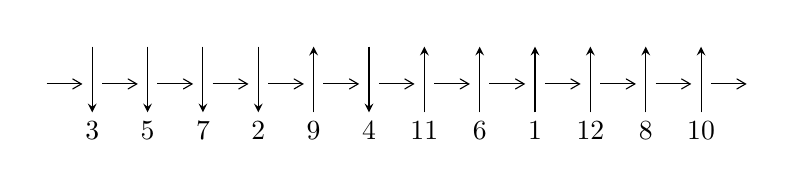
\begin{tikzpicture}[x=20pt, y=17pt]
	% nodes
	\node (C0) at (0, 0) {};
	\node (C1) at (1, 0) {};
	\node (C1U) at (1, +1) {};
	\node (C1D) at (1, -1) {3};

	\node (C2) at (2, 0) {};
	\node (C2U) at (2, +1) {};
	\node (C2D) at (2, -1) {5};

	\node (C3) at (3, 0) {};
	\node (C3U) at (3, +1) {};
	\node (C3D) at (3, -1) {7};

	\node (C4) at (4, 0) {};
	\node (C4U) at (4, +1) {};
	\node (C4D) at (4, -1) {2};

	\node (C5) at (5, 0) {};
	\node (C5U) at (5, +1) {};
	\node (C5D) at (5, -1) {9};

	\node (C6) at (6, 0) {};
	\node (C6U) at (6, +1) {};
	\node (C6D) at (6, -1) {4};

	\node (C7) at (7, 0) {};
	\node (C7U) at (7, +1) {};
	\node (C7D) at (7, -1) {11};

	\node (C8) at (8, 0) {};
	\node (C8U) at (8, +1) {};
	\node (C8D) at (8, -1) {6};

	\node (C9) at (9, 0) {};
	\node (C9U) at (9, +1) {};
	\node (C9D) at (9, -1) {1};

	\node (C10) at (10, 0) {};
	\node (C10U) at (10, +1) {};
	\node (C10D) at (10, -1) {12};

	\node (C11) at (11, 0) {};
	\node (C11U) at (11, +1) {};
	\node (C11D) at (11, -1) {8};

	\node (C12) at (12, 0) {};
	\node (C12U) at (12, +1) {};
	\node (C12D) at (12, -1) {10};
	\node (C13) at (13, 0) {};

	% arrows
	\draw[->,>={angle 60}]
	(C0) edge (C1) (C1) edge (C2) (C2) edge (C3) (C3) edge (C4) (C4) edge (C5) (C5) edge (C6) (C6) edge (C7) (C7) edge (C8) (C8) edge (C9) (C9) edge (C10) (C10) edge (C11) (C11) edge (C12) (C12) edge (C13) ;	\draw[->,>=stealth]
	(C1U) edge (C1D) (C2U) edge (C2D) (C3U) edge (C3D) (C4U) edge (C4D) (C5D) edge (C5U) (C6U) edge (C6D) (C7D) edge (C7U) (C8D) edge (C8U) (C9D) edge (C9U) (C10D) edge (C10U) (C11D) edge (C11U) (C12D) edge (C12U) ;
	\end{tikzpicture} \\
\hhline{~~} \\& 
\textbf{Solving Sequence} \\ \cline{2-2} 
 &
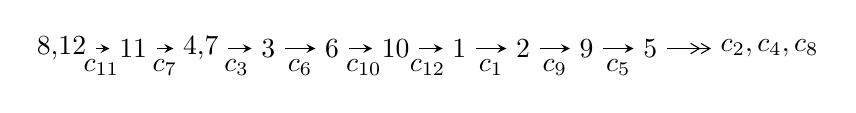
\begin{tikzpicture}[x=23pt, y=7pt]
	% node
	\node (A0) at (-1/8, 0) {8,12};
	\node (A1) at (1, 0) {11};
	\node (A2) at (33/16, 0) {4,7};
	\node (A3) at (25/8, 0) {3};
	\node (A4) at (33/8, 0) {6};
	\node (A5) at (41/8, 0) {10};
	\node (A6) at (49/8, 0) {1};
	\node (A7) at (57/8, 0) {2};
	\node (A8) at (65/8, 0) {9};
	\node (A9) at (73/8, 0) {5};
	\node (C1) at (1/2, -1) {$c_{11}$};
	\node (C2) at (3/2, -1) {$c_{7}$};
	\node (C3) at (21/8, -1) {$c_{3}$};
	\node (C4) at (29/8, -1) {$c_{6}$};
	\node (C5) at (37/8, -1) {$c_{10}$};
	\node (C6) at (45/8, -1) {$c_{12}$};
	\node (C7) at (53/8, -1) {$c_{1}$};
	\node (C8) at (61/8, -1) {$c_{9}$};
	\node (C9) at (69/8, -1) {$c_{5}$};
	\node (A10) at (11, 0) {$c_{2},c_{4},c_{8}$};

	% edge
	\draw[->,>=stealth]	
	(A0) edge (A1) (A1) edge (A2) (A2) edge (A3) (A3) edge (A4) (A4) edge (A5) (A5) edge (A6) (A6) edge (A7) (A7) edge (A8) (A8) edge (A9) ;
	\draw[->>,>={angle 60}]	
	(A9) edge (A10);
\end{tikzpicture} \\ 

\end{tabular} \\

\footnotetext{
The image of knot diagram is generated by the software ``\textbf{Draw programme}" developed by Andrew Bartholomew(\url{http://www.layer8.co.uk/maths/draw/index.htm\#Running-draw}), where we modified some parts for our purpose(\url{https://github.com/CATsTAILs/LinksPainter}).
}\phantom \\ \newline 
\centering \textbf{Ideals for irreducible components\footnotemark of $X_{\text{par}}$} 
 
\begin{align*}
I^u_{1}&=\langle 
-1.02752\times10^{30} u^{93}+2.82962\times10^{30} u^{92}+\cdots+7.01285\times10^{29} b+2.68128\times10^{30},\\
\phantom{I^u_{1}}&\phantom{= \langle  }1.33287\times10^{30} u^{93}-5.41849\times10^{30} u^{92}+\cdots+2.33762\times10^{29} a-3.96691\times10^{30},\;u^{94}-5 u^{93}+\cdots-15 u+1\rangle \\
I^u_{2}&=\langle 
2 a u- u^2+b+2 a,\;u^2 a+a^2- a u+u^2+u-1,\;u^3+u^2-1\rangle \\
I^u_{3}&=\langle 
- u^4+b-2,\;2 u^4- u^3+a+u+3,\;u^5- u^4+u^2+u-1\rangle \\
I^u_{4}&=\langle 
u^2+b- u,\;- u^2+a- u,\;u^3+u^2-1\rangle \\
\\
\end{align*}
\raggedright * 4 irreducible components of $\dim_{\mathbb{C}}=0$, with total 108 representations.\\
\footnotetext{All coefficients of polynomials are rational numbers. But the coefficients are sometimes approximated in decimal forms when there is not enough margin.}
\newpage
\renewcommand{\arraystretch}{1}
\centering \section*{I. $I^u_{1}= \langle -1.03\times10^{30} u^{93}+2.83\times10^{30} u^{92}+\cdots+7.01\times10^{29} b+2.68\times10^{30},\;1.33\times10^{30} u^{93}-5.42\times10^{30} u^{92}+\cdots+2.34\times10^{29} a-3.97\times10^{30},\;u^{94}-5 u^{93}+\cdots-15 u+1 \rangle$}
\flushleft \textbf{(i) Arc colorings}\\
\begin{tabular}{m{7pt} m{180pt} m{7pt} m{180pt} }
\flushright $a_{8}=$&$\begin{pmatrix}0\\u\end{pmatrix}$ \\
\flushright $a_{12}=$&$\begin{pmatrix}1\\0\end{pmatrix}$ \\
\flushright $a_{11}=$&$\begin{pmatrix}1\\u^2\end{pmatrix}$ \\
\flushright $a_{4}=$&$\begin{pmatrix}-5.70183 u^{93}+23.1795 u^{92}+\cdots-124.011 u+16.9699\\1.46519 u^{93}-4.03491 u^{92}+\cdots+39.3234 u-3.82338\end{pmatrix}$ \\
\flushright $a_{7}=$&$\begin{pmatrix}- u\\- u^3+u\end{pmatrix}$ \\
\flushright $a_{3}=$&$\begin{pmatrix}-2.89290 u^{93}+5.89251 u^{92}+\cdots-52.1238 u+11.9968\\-12.2961 u^{93}+52.5426 u^{92}+\cdots-84.0089 u+4.39211\end{pmatrix}$ \\
\flushright $a_{6}=$&$\begin{pmatrix}-6.77410 u^{93}+35.7202 u^{92}+\cdots-163.016 u+15.4696\\20.9419 u^{93}-88.1661 u^{92}+\cdots+226.524 u-15.8512\end{pmatrix}$ \\
\flushright $a_{10}=$&$\begin{pmatrix}- u^2+1\\u^2\end{pmatrix}$ \\
\flushright $a_{1}=$&$\begin{pmatrix}u^4- u^2+1\\- u^4\end{pmatrix}$ \\
\flushright $a_{2}=$&$\begin{pmatrix}5.35996 u^{93}-24.6779 u^{92}+\cdots+130.166 u-14.0247\\-9.43706 u^{93}+37.3806 u^{92}+\cdots-111.393 u+8.46972\end{pmatrix}$ \\
\flushright $a_{9}=$&$\begin{pmatrix}- u^6+u^4-2 u^2+1\\u^6+u^2\end{pmatrix}$ \\
\flushright $a_{5}=$&$\begin{pmatrix}-1.23353 u^{93}+0.892677 u^{92}+\cdots-10.5212 u+5.01394\\-6.25844 u^{93}+27.0384 u^{92}+\cdots-59.6741 u+3.69409\end{pmatrix}$\\&\end{tabular}
\flushleft \textbf{(ii) Obstruction class $= -1$}\\~\\
\flushleft \textbf{(iii) Cusp Shapes $= 6.58579 u^{93}-34.2762 u^{92}+\cdots+276.933 u-31.2371$}\\~\\
\newpage\renewcommand{\arraystretch}{1}
\flushleft \textbf{(iv) u-Polynomials at the component}\newline \\
\begin{tabular}{m{50pt}|m{274pt}}
Crossings & \hspace{64pt}u-Polynomials at each crossing \\
\hline $$\begin{aligned}c_{1}\end{aligned}$$&$\begin{aligned}
&u^{94}+47 u^{93}+\cdots+2083 u+1
\end{aligned}$\\
\hline $$\begin{aligned}c_{2},c_{4}\end{aligned}$$&$\begin{aligned}
&u^{94}-9 u^{93}+\cdots+37 u+1
\end{aligned}$\\
\hline $$\begin{aligned}c_{3},c_{6}\end{aligned}$$&$\begin{aligned}
&u^{94}-4 u^{93}+\cdots+320 u-32
\end{aligned}$\\
\hline $$\begin{aligned}c_{5},c_{8}\end{aligned}$$&$\begin{aligned}
&u^{94}+2 u^{93}+\cdots-2560 u-512
\end{aligned}$\\
\hline $$\begin{aligned}c_{7},c_{11}\end{aligned}$$&$\begin{aligned}
&u^{94}-5 u^{93}+\cdots-15 u+1
\end{aligned}$\\
\hline $$\begin{aligned}c_{9},c_{10},c_{12}\end{aligned}$$&$\begin{aligned}
&u^{94}-23 u^{93}+\cdots-185 u+1
\end{aligned}$\\
\hline
\end{tabular}\\~\\
\newpage\renewcommand{\arraystretch}{1}
\flushleft \textbf{(v) Riley Polynomials at the component}\newline \\
\begin{tabular}{m{50pt}|m{274pt}}
Crossings & \hspace{64pt}Riley Polynomials at each crossing \\
\hline $$\begin{aligned}c_{1}\end{aligned}$$&$\begin{aligned}
&y^{94}+9 y^{93}+\cdots-4301459 y+1
\end{aligned}$\\
\hline $$\begin{aligned}c_{2},c_{4}\end{aligned}$$&$\begin{aligned}
&y^{94}-47 y^{93}+\cdots-2083 y+1
\end{aligned}$\\
\hline $$\begin{aligned}c_{3},c_{6}\end{aligned}$$&$\begin{aligned}
&y^{94}+42 y^{93}+\cdots-37376 y+1024
\end{aligned}$\\
\hline $$\begin{aligned}c_{5},c_{8}\end{aligned}$$&$\begin{aligned}
&y^{94}+56 y^{93}+\cdots+3801088 y+262144
\end{aligned}$\\
\hline $$\begin{aligned}c_{7},c_{11}\end{aligned}$$&$\begin{aligned}
&y^{94}-23 y^{93}+\cdots-185 y+1
\end{aligned}$\\
\hline $$\begin{aligned}c_{9},c_{10},c_{12}\end{aligned}$$&$\begin{aligned}
&y^{94}+101 y^{93}+\cdots-28969 y+1
\end{aligned}$\\
\hline
\end{tabular}\\~\\
\newpage\flushleft \textbf{(vi) Complex Volumes and Cusp Shapes}
$$\begin{array}{c|c|c}  
\text{Solutions to }I^u_{1}& \I (\text{vol} + \sqrt{-1}CS) & \text{Cusp shape}\\
 \hline 
\begin{aligned}
u &= -0.905451 + 0.437078 I \\
a &= -0.38908 - 2.12552 I \\
b &= -1.55661 + 2.03416 I\end{aligned}
 & -2.95530 - 3.62965 I & \phantom{-0.000000 } 0 \\ \hline\begin{aligned}
u &= -0.905451 - 0.437078 I \\
a &= -0.38908 + 2.12552 I \\
b &= -1.55661 - 2.03416 I\end{aligned}
 & -2.95530 + 3.62965 I & \phantom{-0.000000 } 0 \\ \hline\begin{aligned}
u &= \phantom{-}0.998868 + 0.153287 I \\
a &= -0.34700 - 1.43569 I \\
b &= \phantom{-}0.933069 + 0.889689 I\end{aligned}
 & \phantom{-}3.69183 - 0.90668 I & \phantom{-0.000000 } 0 \\ \hline\begin{aligned}
u &= \phantom{-}0.998868 - 0.153287 I \\
a &= -0.34700 + 1.43569 I \\
b &= \phantom{-}0.933069 - 0.889689 I\end{aligned}
 & \phantom{-}3.69183 + 0.90668 I & \phantom{-0.000000 } 0 \\ \hline\begin{aligned}
u &= \phantom{-}0.885560 + 0.419384 I \\
a &= \phantom{-}0.739482 + 1.067380 I \\
b &= -1.14651 - 1.15035 I\end{aligned}
 & \phantom{-}2.64492 + 6.49916 I & \phantom{-0.000000 } 0 \\ \hline\begin{aligned}
u &= \phantom{-}0.885560 - 0.419384 I \\
a &= \phantom{-}0.739482 - 1.067380 I \\
b &= -1.14651 + 1.15035 I\end{aligned}
 & \phantom{-}2.64492 - 6.49916 I & \phantom{-0.000000 } 0 \\ \hline\begin{aligned}
u &= \phantom{-}0.913302 + 0.325477 I \\
a &= -0.70472 - 1.26351 I \\
b &= \phantom{-}1.10966 + 1.07964 I\end{aligned}
 & \phantom{-}4.12929 + 1.39857 I & \phantom{-0.000000 } 0 \\ \hline\begin{aligned}
u &= \phantom{-}0.913302 - 0.325477 I \\
a &= -0.70472 + 1.26351 I \\
b &= \phantom{-}1.10966 - 1.07964 I\end{aligned}
 & \phantom{-}4.12929 - 1.39857 I & \phantom{-0.000000 } 0 \\ \hline\begin{aligned}
u &= -0.954895 + 0.414756 I \\
a &= -0.025203 + 0.334361 I \\
b &= \phantom{-}1.332920 - 0.124333 I\end{aligned}
 & -2.18704 - 6.14689 I & \phantom{-0.000000 } 0 \\ \hline\begin{aligned}
u &= -0.954895 - 0.414756 I \\
a &= -0.025203 - 0.334361 I \\
b &= \phantom{-}1.332920 + 0.124333 I\end{aligned}
 & -2.18704 + 6.14689 I & \phantom{-0.000000 } 0\\
 \hline 
 \end{array}$$\newpage$$\begin{array}{c|c|c}  
\text{Solutions to }I^u_{1}& \I (\text{vol} + \sqrt{-1}CS) & \text{Cusp shape}\\
 \hline 
\begin{aligned}
u &= -0.721866 + 0.754158 I \\
a &= \phantom{-}0.693424 - 0.277978 I \\
b &= -0.545353 - 0.989217 I\end{aligned}
 & -2.17526 - 1.45322 I & \phantom{-0.000000 } 0 \\ \hline\begin{aligned}
u &= -0.721866 - 0.754158 I \\
a &= \phantom{-}0.693424 + 0.277978 I \\
b &= -0.545353 + 0.989217 I\end{aligned}
 & -2.17526 + 1.45322 I & \phantom{-0.000000 } 0 \\ \hline\begin{aligned}
u &= \phantom{-}1.056890 + 0.104571 I \\
a &= \phantom{-}0.232763 + 1.345440 I \\
b &= -0.915683 - 0.763709 I\end{aligned}
 & \phantom{-}1.69927 - 5.76809 I & \phantom{-0.000000 } 0 \\ \hline\begin{aligned}
u &= \phantom{-}1.056890 - 0.104571 I \\
a &= \phantom{-}0.232763 - 1.345440 I \\
b &= -0.915683 + 0.763709 I\end{aligned}
 & \phantom{-}1.69927 + 5.76809 I & \phantom{-0.000000 } 0 \\ \hline\begin{aligned}
u &= -0.995318 + 0.375431 I \\
a &= \phantom{-}0.18189 + 1.71349 I \\
b &= \phantom{-}1.16693 - 1.59065 I\end{aligned}
 & \phantom{-}2.38179 - 6.85574 I & \phantom{-0.000000 } 0 \\ \hline\begin{aligned}
u &= -0.995318 - 0.375431 I \\
a &= \phantom{-}0.18189 - 1.71349 I \\
b &= \phantom{-}1.16693 + 1.59065 I\end{aligned}
 & \phantom{-}2.38179 + 6.85574 I & \phantom{-0.000000 } 0 \\ \hline\begin{aligned}
u &= -0.511330 + 0.782712 I \\
a &= -0.547011 + 0.562475 I \\
b &= \phantom{-}0.713250 + 0.726812 I\end{aligned}
 & -4.15606 - 4.95399 I & \phantom{-0.000000 } 0 \\ \hline\begin{aligned}
u &= -0.511330 - 0.782712 I \\
a &= -0.547011 - 0.562475 I \\
b &= \phantom{-}0.713250 - 0.726812 I\end{aligned}
 & -4.15606 + 4.95399 I & \phantom{-0.000000 } 0 \\ \hline\begin{aligned}
u &= \phantom{-}0.929009 + 0.068800 I \\
a &= -0.26626 - 1.43751 I \\
b &= -0.492725 + 0.646944 I\end{aligned}
 & -0.254266 - 0.867513 I & \phantom{-0.000000 } 0 \\ \hline\begin{aligned}
u &= \phantom{-}0.929009 - 0.068800 I \\
a &= -0.26626 + 1.43751 I \\
b &= -0.492725 - 0.646944 I\end{aligned}
 & -0.254266 + 0.867513 I & \phantom{-0.000000 } 0\\
 \hline 
 \end{array}$$\newpage$$\begin{array}{c|c|c}  
\text{Solutions to }I^u_{1}& \I (\text{vol} + \sqrt{-1}CS) & \text{Cusp shape}\\
 \hline 
\begin{aligned}
u &= -0.823707 + 0.383516 I \\
a &= -0.041446 - 0.332414 I \\
b &= -1.142000 - 0.123519 I\end{aligned}
 & -0.67738 - 1.92321 I & \phantom{-0.000000 } 0 \\ \hline\begin{aligned}
u &= -0.823707 - 0.383516 I \\
a &= -0.041446 + 0.332414 I \\
b &= -1.142000 + 0.123519 I\end{aligned}
 & -0.67738 + 1.92321 I & \phantom{-0.000000 } 0 \\ \hline\begin{aligned}
u &= -1.036230 + 0.405152 I \\
a &= -0.04234 - 1.71265 I \\
b &= -1.23040 + 1.38676 I\end{aligned}
 & -0.10577 - 12.27470 I & \phantom{-0.000000 } 0 \\ \hline\begin{aligned}
u &= -1.036230 - 0.405152 I \\
a &= -0.04234 + 1.71265 I \\
b &= -1.23040 - 1.38676 I\end{aligned}
 & -0.10577 + 12.27470 I & \phantom{-0.000000 } 0 \\ \hline\begin{aligned}
u &= -0.859284 + 0.214626 I \\
a &= \phantom{-}0.548445 + 1.203540 I \\
b &= \phantom{-}0.64460 - 2.02449 I\end{aligned}
 & \phantom{-}4.79944 - 3.38706 I & \phantom{-0.000000 -}0. + 9.66029 I \\ \hline\begin{aligned}
u &= -0.859284 - 0.214626 I \\
a &= \phantom{-}0.548445 - 1.203540 I \\
b &= \phantom{-}0.64460 + 2.02449 I\end{aligned}
 & \phantom{-}4.79944 + 3.38706 I & \phantom{-0.000000 } 0. - 9.66029 I \\ \hline\begin{aligned}
u &= -0.878091 + 0.732966 I \\
a &= \phantom{-}2.13662 - 2.26977 I \\
b &= -4.27115 - 0.73401 I\end{aligned}
 & -4.29337 - 2.79203 I & \phantom{-0.000000 } 0 \\ \hline\begin{aligned}
u &= -0.878091 - 0.732966 I \\
a &= \phantom{-}2.13662 + 2.26977 I \\
b &= -4.27115 + 0.73401 I\end{aligned}
 & -4.29337 + 2.79203 I & \phantom{-0.000000 } 0 \\ \hline\begin{aligned}
u &= \phantom{-}0.792347 + 0.274736 I \\
a &= \phantom{-}0.600358 + 1.032710 I \\
b &= \phantom{-}0.263529 - 0.187085 I\end{aligned}
 & -0.12060 + 1.76624 I & \phantom{-}2.00000 - 5.30326 I \\ \hline\begin{aligned}
u &= \phantom{-}0.792347 - 0.274736 I \\
a &= \phantom{-}0.600358 - 1.032710 I \\
b &= \phantom{-}0.263529 + 0.187085 I\end{aligned}
 & -0.12060 - 1.76624 I & \phantom{-}2.00000 + 5.30326 I\\
 \hline 
 \end{array}$$\newpage$$\begin{array}{c|c|c}  
\text{Solutions to }I^u_{1}& \I (\text{vol} + \sqrt{-1}CS) & \text{Cusp shape}\\
 \hline 
\begin{aligned}
u &= -0.995387 + 0.608742 I \\
a &= -0.063080 + 0.575346 I \\
b &= \phantom{-}1.46287 - 0.61224 I\end{aligned}
 & -2.64588 - 0.14652 I & \phantom{-0.000000 } 0 \\ \hline\begin{aligned}
u &= -0.995387 - 0.608742 I \\
a &= -0.063080 - 0.575346 I \\
b &= \phantom{-}1.46287 + 0.61224 I\end{aligned}
 & -2.64588 + 0.14652 I & \phantom{-0.000000 } 0 \\ \hline\begin{aligned}
u &= -0.844120 + 0.835558 I \\
a &= \phantom{-}1.108580 - 0.589162 I \\
b &= -1.15995 - 1.20057 I\end{aligned}
 & -3.06674 - 1.11761 I & \phantom{-0.000000 } 0 \\ \hline\begin{aligned}
u &= -0.844120 - 0.835558 I \\
a &= \phantom{-}1.108580 + 0.589162 I \\
b &= -1.15995 + 1.20057 I\end{aligned}
 & -3.06674 + 1.11761 I & \phantom{-0.000000 } 0 \\ \hline\begin{aligned}
u &= -0.964903 + 0.705690 I \\
a &= \phantom{-}0.079505 - 0.904415 I \\
b &= -1.75161 + 0.99325 I\end{aligned}
 & -1.44073 - 4.07182 I & \phantom{-0.000000 } 0 \\ \hline\begin{aligned}
u &= -0.964903 - 0.705690 I \\
a &= \phantom{-}0.079505 + 0.904415 I \\
b &= -1.75161 - 0.99325 I\end{aligned}
 & -1.44073 + 4.07182 I & \phantom{-0.000000 } 0 \\ \hline\begin{aligned}
u &= \phantom{-}0.884235 + 0.815291 I \\
a &= \phantom{-}0.997732 - 0.766176 I \\
b &= \phantom{-}1.20106 + 2.96128 I\end{aligned}
 & -1.221240 - 0.245856 I & \phantom{-0.000000 } 0 \\ \hline\begin{aligned}
u &= \phantom{-}0.884235 - 0.815291 I \\
a &= \phantom{-}0.997732 + 0.766176 I \\
b &= \phantom{-}1.20106 - 2.96128 I\end{aligned}
 & -1.221240 + 0.245856 I & \phantom{-0.000000 } 0 \\ \hline\begin{aligned}
u &= -0.227459 + 0.757503 I \\
a &= \phantom{-}1.90723 + 0.28691 I \\
b &= -1.249060 - 0.643882 I\end{aligned}
 & -2.75290 + 8.12923 I & -3.14725 - 5.96002 I \\ \hline\begin{aligned}
u &= -0.227459 - 0.757503 I \\
a &= \phantom{-}1.90723 - 0.28691 I \\
b &= -1.249060 + 0.643882 I\end{aligned}
 & -2.75290 - 8.12923 I & -3.14725 + 5.96002 I\\
 \hline 
 \end{array}$$\newpage$$\begin{array}{c|c|c}  
\text{Solutions to }I^u_{1}& \I (\text{vol} + \sqrt{-1}CS) & \text{Cusp shape}\\
 \hline 
\begin{aligned}
u &= \phantom{-}0.823780 + 0.888088 I \\
a &= \phantom{-}1.65148 - 0.04048 I \\
b &= -0.63909 + 2.70840 I\end{aligned}
 & -5.87040 - 4.86160 I & \phantom{-0.000000 } 0 \\ \hline\begin{aligned}
u &= \phantom{-}0.823780 - 0.888088 I \\
a &= \phantom{-}1.65148 + 0.04048 I \\
b &= -0.63909 - 2.70840 I\end{aligned}
 & -5.87040 + 4.86160 I & \phantom{-0.000000 } 0 \\ \hline\begin{aligned}
u &= -0.888709 + 0.828883 I \\
a &= -0.97034 + 1.31401 I \\
b &= \phantom{-}2.74854 - 0.53626 I\end{aligned}
 & -6.59016 - 1.87331 I & \phantom{-0.000000 } 0 \\ \hline\begin{aligned}
u &= -0.888709 - 0.828883 I \\
a &= -0.97034 - 1.31401 I \\
b &= \phantom{-}2.74854 + 0.53626 I\end{aligned}
 & -6.59016 + 1.87331 I & \phantom{-0.000000 } 0 \\ \hline\begin{aligned}
u &= -0.768651 + 0.153462 I \\
a &= -0.662957 - 0.821078 I \\
b &= -0.62346 + 2.12671 I\end{aligned}
 & \phantom{-}4.22053 + 2.42602 I & \phantom{-}4.48189 + 9.29126 I \\ \hline\begin{aligned}
u &= -0.768651 - 0.153462 I \\
a &= -0.662957 + 0.821078 I \\
b &= -0.62346 - 2.12671 I\end{aligned}
 & \phantom{-}4.22053 - 2.42602 I & \phantom{-}4.48189 - 9.29126 I \\ \hline\begin{aligned}
u &= \phantom{-}0.911045 + 0.807605 I \\
a &= -0.744831 + 1.036970 I \\
b &= -1.67892 - 2.96867 I\end{aligned}
 & -1.13789 + 6.32136 I & \phantom{-0.000000 } 0 \\ \hline\begin{aligned}
u &= \phantom{-}0.911045 - 0.807605 I \\
a &= -0.744831 - 1.036970 I \\
b &= -1.67892 + 2.96867 I\end{aligned}
 & -1.13789 - 6.32136 I & \phantom{-0.000000 } 0 \\ \hline\begin{aligned}
u &= \phantom{-}0.817206 + 0.911898 I \\
a &= -1.71283 - 0.11928 I \\
b &= \phantom{-}1.01533 - 2.55879 I\end{aligned}
 & -8.86590 - 10.56170 I & \phantom{-0.000000 } 0 \\ \hline\begin{aligned}
u &= \phantom{-}0.817206 - 0.911898 I \\
a &= -1.71283 + 0.11928 I \\
b &= \phantom{-}1.01533 + 2.55879 I\end{aligned}
 & -8.86590 + 10.56170 I & \phantom{-0.000000 } 0\\
 \hline 
 \end{array}$$\newpage$$\begin{array}{c|c|c}  
\text{Solutions to }I^u_{1}& \I (\text{vol} + \sqrt{-1}CS) & \text{Cusp shape}\\
 \hline 
\begin{aligned}
u &= \phantom{-}0.845161 + 0.889434 I \\
a &= -0.288648 - 0.032497 I \\
b &= \phantom{-}0.104224 + 0.631601 I\end{aligned}
 & -10.59930 - 3.58899 I & \phantom{-0.000000 } 0 \\ \hline\begin{aligned}
u &= \phantom{-}0.845161 - 0.889434 I \\
a &= -0.288648 + 0.032497 I \\
b &= \phantom{-}0.104224 - 0.631601 I\end{aligned}
 & -10.59930 + 3.58899 I & \phantom{-0.000000 } 0 \\ \hline\begin{aligned}
u &= -0.913525 + 0.821468 I \\
a &= -1.23296 + 0.92411 I \\
b &= \phantom{-}1.62458 + 1.03417 I\end{aligned}
 & -6.51331 - 4.28654 I & \phantom{-0.000000 } 0 \\ \hline\begin{aligned}
u &= -0.913525 - 0.821468 I \\
a &= -1.23296 - 0.92411 I \\
b &= \phantom{-}1.62458 - 1.03417 I\end{aligned}
 & -6.51331 + 4.28654 I & \phantom{-0.000000 } 0 \\ \hline\begin{aligned}
u &= \phantom{-}0.873838 + 0.868456 I \\
a &= \phantom{-}0.240797 + 0.078349 I \\
b &= \phantom{-}0.061011 - 0.590277 I\end{aligned}
 & -8.40697 + 1.63722 I & \phantom{-0.000000 } 0 \\ \hline\begin{aligned}
u &= \phantom{-}0.873838 - 0.868456 I \\
a &= \phantom{-}0.240797 - 0.078349 I \\
b &= \phantom{-}0.061011 + 0.590277 I\end{aligned}
 & -8.40697 - 1.63722 I & \phantom{-0.000000 } 0 \\ \hline\begin{aligned}
u &= \phantom{-}0.860026 + 0.884880 I \\
a &= -1.88264 + 0.33095 I \\
b &= \phantom{-}0.51218 - 3.50291 I\end{aligned}
 & -11.31680 - 0.57038 I & \phantom{-0.000000 } 0 \\ \hline\begin{aligned}
u &= \phantom{-}0.860026 - 0.884880 I \\
a &= -1.88264 - 0.33095 I \\
b &= \phantom{-}0.51218 + 3.50291 I\end{aligned}
 & -11.31680 + 0.57038 I & \phantom{-0.000000 } 0 \\ \hline\begin{aligned}
u &= -0.865887 + 0.882160 I \\
a &= -0.996542 + 0.730783 I \\
b &= \phantom{-}1.20983 + 0.96608 I\end{aligned}
 & -5.55893 + 3.28453 I & \phantom{-0.000000 } 0 \\ \hline\begin{aligned}
u &= -0.865887 - 0.882160 I \\
a &= -0.996542 - 0.730783 I \\
b &= \phantom{-}1.20983 - 0.96608 I\end{aligned}
 & -5.55893 - 3.28453 I & \phantom{-0.000000 } 0\\
 \hline 
 \end{array}$$\newpage$$\begin{array}{c|c|c}  
\text{Solutions to }I^u_{1}& \I (\text{vol} + \sqrt{-1}CS) & \text{Cusp shape}\\
 \hline 
\begin{aligned}
u &= -0.946485 + 0.806200 I \\
a &= \phantom{-}0.601050 - 1.153690 I \\
b &= -2.39169 + 0.76305 I\end{aligned}
 & -2.75258 - 5.01184 I & \phantom{-0.000000 } 0 \\ \hline\begin{aligned}
u &= -0.946485 - 0.806200 I \\
a &= \phantom{-}0.601050 + 1.153690 I \\
b &= -2.39169 - 0.76305 I\end{aligned}
 & -2.75258 + 5.01184 I & \phantom{-0.000000 } 0 \\ \hline\begin{aligned}
u &= -0.536657 + 0.519170 I \\
a &= \phantom{-}0.199660 - 0.585956 I \\
b &= -0.726972 - 0.579075 I\end{aligned}
 & -1.58168 - 1.49511 I & -1.20774 + 4.62157 I \\ \hline\begin{aligned}
u &= -0.536657 - 0.519170 I \\
a &= \phantom{-}0.199660 + 0.585956 I \\
b &= -0.726972 + 0.579075 I\end{aligned}
 & -1.58168 + 1.49511 I & -1.20774 - 4.62157 I \\ \hline\begin{aligned}
u &= \phantom{-}0.945080 + 0.838821 I \\
a &= \phantom{-}0.142467 + 0.191244 I \\
b &= \phantom{-}0.447571 - 0.324800 I\end{aligned}
 & -8.18097 + 4.69776 I & \phantom{-0.000000 } 0 \\ \hline\begin{aligned}
u &= \phantom{-}0.945080 - 0.838821 I \\
a &= \phantom{-}0.142467 - 0.191244 I \\
b &= \phantom{-}0.447571 + 0.324800 I\end{aligned}
 & -8.18097 - 4.69776 I & \phantom{-0.000000 } 0 \\ \hline\begin{aligned}
u &= -0.391118 + 0.616467 I \\
a &= \phantom{-}2.19814 + 0.27289 I \\
b &= -1.22053 - 1.25849 I\end{aligned}
 & -4.57237 - 0.27043 I & -5.36990 - 0.41408 I \\ \hline\begin{aligned}
u &= -0.391118 - 0.616467 I \\
a &= \phantom{-}2.19814 - 0.27289 I \\
b &= -1.22053 + 1.25849 I\end{aligned}
 & -4.57237 + 0.27043 I & -5.36990 + 0.41408 I \\ \hline\begin{aligned}
u &= -0.958623 + 0.842313 I \\
a &= -0.725274 + 1.015570 I \\
b &= \phantom{-}2.36009 - 0.57501 I\end{aligned}
 & -5.26401 - 9.67296 I & \phantom{-0.000000 } 0 \\ \hline\begin{aligned}
u &= -0.958623 - 0.842313 I \\
a &= -0.725274 - 1.015570 I \\
b &= \phantom{-}2.36009 + 0.57501 I\end{aligned}
 & -5.26401 + 9.67296 I & \phantom{-0.000000 } 0\\
 \hline 
 \end{array}$$\newpage$$\begin{array}{c|c|c}  
\text{Solutions to }I^u_{1}& \I (\text{vol} + \sqrt{-1}CS) & \text{Cusp shape}\\
 \hline 
\begin{aligned}
u &= \phantom{-}0.963009 + 0.840863 I \\
a &= \phantom{-}0.36986 - 1.89136 I \\
b &= \phantom{-}3.04124 + 2.99193 I\end{aligned}
 & -10.99000 + 6.96104 I & \phantom{-0.000000 } 0 \\ \hline\begin{aligned}
u &= \phantom{-}0.963009 - 0.840863 I \\
a &= \phantom{-}0.36986 + 1.89136 I \\
b &= \phantom{-}3.04124 - 2.99193 I\end{aligned}
 & -10.99000 - 6.96104 I & \phantom{-0.000000 } 0 \\ \hline\begin{aligned}
u &= \phantom{-}0.984748 + 0.822057 I \\
a &= -0.07028 + 1.64656 I \\
b &= -2.82195 - 2.36983 I\end{aligned}
 & -5.36286 + 11.19750 I & \phantom{-0.000000 } 0 \\ \hline\begin{aligned}
u &= \phantom{-}0.984748 - 0.822057 I \\
a &= -0.07028 - 1.64656 I \\
b &= -2.82195 + 2.36983 I\end{aligned}
 & -5.36286 - 11.19750 I & \phantom{-0.000000 } 0 \\ \hline\begin{aligned}
u &= \phantom{-}0.974104 + 0.834723 I \\
a &= -0.113786 - 0.235277 I \\
b &= -0.526723 + 0.214120 I\end{aligned}
 & -10.1908 + 9.9724 I & \phantom{-0.000000 } 0 \\ \hline\begin{aligned}
u &= \phantom{-}0.974104 - 0.834723 I \\
a &= -0.113786 + 0.235277 I \\
b &= -0.526723 - 0.214120 I\end{aligned}
 & -10.1908 - 9.9724 I & \phantom{-0.000000 } 0 \\ \hline\begin{aligned}
u &= -0.308065 + 0.638255 I \\
a &= -0.510667 + 0.784027 I \\
b &= \phantom{-}0.745034 + 0.663909 I\end{aligned}
 & -4.22284 + 2.28384 I & -5.40942 - 1.60159 I \\ \hline\begin{aligned}
u &= -0.308065 - 0.638255 I \\
a &= -0.510667 - 0.784027 I \\
b &= \phantom{-}0.745034 - 0.663909 I\end{aligned}
 & -4.22284 - 2.28384 I & -5.40942 + 1.60159 I \\ \hline\begin{aligned}
u &= \phantom{-}0.911762 + 0.918432 I \\
a &= -0.149456 + 0.035449 I \\
b &= \phantom{-}0.118572 + 0.297180 I\end{aligned}
 & -13.05620 + 3.87938 I & \phantom{-0.000000 } 0 \\ \hline\begin{aligned}
u &= \phantom{-}0.911762 - 0.918432 I \\
a &= -0.149456 - 0.035449 I \\
b &= \phantom{-}0.118572 - 0.297180 I\end{aligned}
 & -13.05620 - 3.87938 I & \phantom{-0.000000 } 0\\
 \hline 
 \end{array}$$\newpage$$\begin{array}{c|c|c}  
\text{Solutions to }I^u_{1}& \I (\text{vol} + \sqrt{-1}CS) & \text{Cusp shape}\\
 \hline 
\begin{aligned}
u &= \phantom{-}1.000930 + 0.829713 I \\
a &= -0.09785 - 1.69655 I \\
b &= \phantom{-}2.99495 + 2.10759 I\end{aligned}
 & -8.2816 + 16.9931 I & \phantom{-0.000000 } 0 \\ \hline\begin{aligned}
u &= \phantom{-}1.000930 - 0.829713 I \\
a &= -0.09785 + 1.69655 I \\
b &= \phantom{-}2.99495 - 2.10759 I\end{aligned}
 & -8.2816 - 16.9931 I & \phantom{-0.000000 } 0 \\ \hline\begin{aligned}
u &= \phantom{-}0.430117 + 0.545073 I \\
a &= \phantom{-}1.23174 + 0.88326 I \\
b &= -0.297726 + 0.130654 I\end{aligned}
 & \phantom{-}1.21330 - 2.82397 I & \phantom{-}1.38406 + 2.73602 I \\ \hline\begin{aligned}
u &= \phantom{-}0.430117 - 0.545073 I \\
a &= \phantom{-}1.23174 - 0.88326 I \\
b &= -0.297726 - 0.130654 I\end{aligned}
 & \phantom{-}1.21330 + 2.82397 I & \phantom{-}1.38406 - 2.73602 I \\ \hline\begin{aligned}
u &= -0.201484 + 0.659185 I \\
a &= -1.98860 - 0.38825 I \\
b &= \phantom{-}1.034070 + 0.728447 I\end{aligned}
 & -0.11479 + 3.13185 I & -0.06207 - 2.62342 I \\ \hline\begin{aligned}
u &= -0.201484 - 0.659185 I \\
a &= -1.98860 + 0.38825 I \\
b &= \phantom{-}1.034070 - 0.728447 I\end{aligned}
 & -0.11479 - 3.13185 I & -0.06207 + 2.62342 I \\ \hline\begin{aligned}
u &= \phantom{-}0.671898 + 0.151886 I \\
a &= \phantom{-}2.07226 + 2.12966 I \\
b &= -1.39171 - 1.41963 I\end{aligned}
 & -0.854990 + 0.184345 I & \phantom{-}6.5747 - 15.0325 I \\ \hline\begin{aligned}
u &= \phantom{-}0.671898 - 0.151886 I \\
a &= \phantom{-}2.07226 - 2.12966 I \\
b &= -1.39171 + 1.41963 I\end{aligned}
 & -0.854990 - 0.184345 I & \phantom{-}6.5747 + 15.0325 I \\ \hline\begin{aligned}
u &= \phantom{-}0.957675 + 0.896988 I \\
a &= -0.0122210 - 0.1384930 I \\
b &= -0.284882 + 0.043144 I\end{aligned}
 & -12.91010 + 2.80229 I & \phantom{-0.000000 } 0 \\ \hline\begin{aligned}
u &= \phantom{-}0.957675 - 0.896988 I \\
a &= -0.0122210 + 0.1384930 I \\
b &= -0.284882 - 0.043144 I\end{aligned}
 & -12.91010 - 2.80229 I & \phantom{-0.000000 } 0\\
 \hline 
 \end{array}$$\newpage$$\begin{array}{c|c|c}  
\text{Solutions to }I^u_{1}& \I (\text{vol} + \sqrt{-1}CS) & \text{Cusp shape}\\
 \hline 
\begin{aligned}
u &= \phantom{-}0.668467\phantom{ +0.000000I} \\
a &= -0.668479\phantom{ +0.000000I} \\
b &= \phantom{-}0.148148\phantom{ +0.000000I}\end{aligned}
 & \phantom{-}0.907840\phantom{ +0.000000I} & \phantom{-}11.5600\phantom{ +0.000000I} \\ \hline\begin{aligned}
u &= \phantom{-}0.194109 + 0.511596 I \\
a &= -1.65256 - 0.97107 I \\
b &= \phantom{-}0.476294 + 0.186820 I\end{aligned}
 & \phantom{-}1.99178 + 1.65996 I & \phantom{-}2.30944 - 4.12201 I \\ \hline\begin{aligned}
u &= \phantom{-}0.194109 - 0.511596 I \\
a &= -1.65256 + 0.97107 I \\
b &= \phantom{-}0.476294 - 0.186820 I\end{aligned}
 & \phantom{-}1.99178 - 1.65996 I & \phantom{-}2.30944 + 4.12201 I \\ \hline\begin{aligned}
u &= \phantom{-}0.0766424\phantom{ +0.000000I} \\
a &= \phantom{-}7.27869\phantom{ +0.000000I} \\
b &= -0.661524\phantom{ +0.000000I}\end{aligned}
 & -1.20372\phantom{ +0.000000I} & -8.99890\phantom{ +0.000000I}\\
 \hline 
 \end{array}$$\newpage\newpage\renewcommand{\arraystretch}{1}
\centering \section*{II. $I^u_{2}= \langle 2 a u- u^2+b+2 a,\;u^2 a+a^2- a u+u^2+u-1,\;u^3+u^2-1 \rangle$}
\flushleft \textbf{(i) Arc colorings}\\
\begin{tabular}{m{7pt} m{180pt} m{7pt} m{180pt} }
\flushright $a_{8}=$&$\begin{pmatrix}0\\u\end{pmatrix}$ \\
\flushright $a_{12}=$&$\begin{pmatrix}1\\0\end{pmatrix}$ \\
\flushright $a_{11}=$&$\begin{pmatrix}1\\u^2\end{pmatrix}$ \\
\flushright $a_{4}=$&$\begin{pmatrix}a\\-2 a u+u^2-2 a\end{pmatrix}$ \\
\flushright $a_{7}=$&$\begin{pmatrix}- u\\u^2+u-1\end{pmatrix}$ \\
\flushright $a_{3}=$&$\begin{pmatrix}- a u+u^2+u-1\\- a u- u^2-2 a+1\end{pmatrix}$ \\
\flushright $a_{6}=$&$\begin{pmatrix}0\\- u^2 a- a u- u^2-2 u\end{pmatrix}$ \\
\flushright $a_{10}=$&$\begin{pmatrix}- u^2+1\\u^2\end{pmatrix}$ \\
\flushright $a_{1}=$&$\begin{pmatrix}u\\- u^2- u+1\end{pmatrix}$ \\
\flushright $a_{2}=$&$\begin{pmatrix}- a u+u^2+u-1\\-3 u^2- a-2 u+1\end{pmatrix}$ \\
\flushright $a_{9}=$&$\begin{pmatrix}0\\u\end{pmatrix}$ \\
\flushright $a_{5}=$&$\begin{pmatrix}0\\- u^2 a- a u- u^2-2 u\end{pmatrix}$\\&\end{tabular}
\flushleft \textbf{(ii) Obstruction class $= 1$}\\~\\
\flushleft \textbf{(iii) Cusp Shapes $= -2 u^2 a-7 a u-6 u^2-9 a+u+5$}\\~\\
\newpage\renewcommand{\arraystretch}{1}
\flushleft \textbf{(iv) u-Polynomials at the component}\newline \\
\begin{tabular}{m{50pt}|m{274pt}}
Crossings & \hspace{64pt}u-Polynomials at each crossing \\
\hline $$\begin{aligned}c_{1},c_{3},c_{12}\end{aligned}$$&$\begin{aligned}
&(u^3- u^2+2 u-1)^2
\end{aligned}$\\
\hline $$\begin{aligned}c_{2},c_{11}\end{aligned}$$&$\begin{aligned}
&(u^3+u^2-1)^2
\end{aligned}$\\
\hline $$\begin{aligned}c_{4},c_{7}\end{aligned}$$&$\begin{aligned}
&(u^3- u^2+1)^2
\end{aligned}$\\
\hline $$\begin{aligned}c_{5},c_{8}\end{aligned}$$&$\begin{aligned}
&u^6
\end{aligned}$\\
\hline $$\begin{aligned}c_{6},c_{9},c_{10}\end{aligned}$$&$\begin{aligned}
&(u^3+u^2+2 u+1)^2
\end{aligned}$\\
\hline
\end{tabular}\\~\\
\newpage\renewcommand{\arraystretch}{1}
\flushleft \textbf{(v) Riley Polynomials at the component}\newline \\
\begin{tabular}{m{50pt}|m{274pt}}
Crossings & \hspace{64pt}Riley Polynomials at each crossing \\
\hline $$\begin{aligned}c_{1},c_{3},c_{6}\\c_{9},c_{10},c_{12}\end{aligned}$$&$\begin{aligned}
&(y^3+3 y^2+2 y-1)^2
\end{aligned}$\\
\hline $$\begin{aligned}c_{2},c_{4},c_{7}\\c_{11}\end{aligned}$$&$\begin{aligned}
&(y^3- y^2+2 y-1)^2
\end{aligned}$\\
\hline $$\begin{aligned}c_{5},c_{8}\end{aligned}$$&$\begin{aligned}
&y^6
\end{aligned}$\\
\hline
\end{tabular}\\~\\
\newpage\flushleft \textbf{(vi) Complex Volumes and Cusp Shapes}
$$\begin{array}{c|c|c}  
\text{Solutions to }I^u_{2}& \I (\text{vol} + \sqrt{-1}CS) & \text{Cusp shape}\\
 \hline 
\begin{aligned}
u &= -0.877439 + 0.744862 I \\
a &= \phantom{-}0.447279 + 0.744862 I \\
b &= \phantom{-}1.21508 - 2.15605 I\end{aligned}
 & \phantom{-0.000000 } -5.65624 I & \phantom{-}3.29784 + 4.97572 I \\ \hline\begin{aligned}
u &= -0.877439 + 0.744862 I \\
a &= -1.53980 + 1.30714 I \\
b &= \phantom{-}2.53980 + 0.66632 I\end{aligned}
 & -4.13758 - 2.82812 I & \phantom{-}11.29331 + 8.29280 I \\ \hline\begin{aligned}
u &= -0.877439 - 0.744862 I \\
a &= \phantom{-}0.447279 - 0.744862 I \\
b &= \phantom{-}1.21508 + 2.15605 I\end{aligned}
 & \phantom{-0.000000 -}5.65624 I & \phantom{-}3.29784 - 4.97572 I \\ \hline\begin{aligned}
u &= -0.877439 - 0.744862 I \\
a &= -1.53980 - 1.30714 I \\
b &= \phantom{-}2.53980 - 0.66632 I\end{aligned}
 & -4.13758 + 2.82812 I & \phantom{-}11.29331 - 8.29280 I \\ \hline\begin{aligned}
u &= \phantom{-}0.754878\phantom{ +0.000000I} \\
a &= \phantom{-}0.092519 + 0.562280 I \\
b &= \phantom{-}0.24512 - 1.97346 I\end{aligned}
 & \phantom{-}4.13758 + 2.82812 I & \phantom{-}0.90884 - 8.67250 I \\ \hline\begin{aligned}
u &= \phantom{-}0.754878\phantom{ +0.000000I} \\
a &= \phantom{-}0.092519 - 0.562280 I \\
b &= \phantom{-}0.24512 + 1.97346 I\end{aligned}
 & \phantom{-}4.13758 - 2.82812 I & \phantom{-}0.90884 + 8.67250 I\\
 \hline 
 \end{array}$$\newpage\newpage\renewcommand{\arraystretch}{1}
\centering \section*{III. $I^u_{3}= \langle - u^4+b-2,\;2 u^4- u^3+a+u+3,\;u^5- u^4+u^2+u-1 \rangle$}
\flushleft \textbf{(i) Arc colorings}\\
\begin{tabular}{m{7pt} m{180pt} m{7pt} m{180pt} }
\flushright $a_{8}=$&$\begin{pmatrix}0\\u\end{pmatrix}$ \\
\flushright $a_{12}=$&$\begin{pmatrix}1\\0\end{pmatrix}$ \\
\flushright $a_{11}=$&$\begin{pmatrix}1\\u^2\end{pmatrix}$ \\
\flushright $a_{4}=$&$\begin{pmatrix}-2 u^4+u^3- u-3\\u^4+2\end{pmatrix}$ \\
\flushright $a_{7}=$&$\begin{pmatrix}- u\\- u^3+u\end{pmatrix}$ \\
\flushright $a_{3}=$&$\begin{pmatrix}-2 u^4+u^3- u-3\\u^4+2\end{pmatrix}$ \\
\flushright $a_{6}=$&$\begin{pmatrix}- u\\- u^3+u\end{pmatrix}$ \\
\flushright $a_{10}=$&$\begin{pmatrix}- u^2+1\\u^2\end{pmatrix}$ \\
\flushright $a_{1}=$&$\begin{pmatrix}u^4- u^2+1\\- u^4\end{pmatrix}$ \\
\flushright $a_{2}=$&$\begin{pmatrix}- u^4+u^3- u^2- u-2\\2\end{pmatrix}$ \\
\flushright $a_{9}=$&$\begin{pmatrix}u^3\\u^4- u^3- u^2+1\end{pmatrix}$ \\
\flushright $a_{5}=$&$\begin{pmatrix}- u^4+u^2-1\\u^4\end{pmatrix}$\\&\end{tabular}
\flushleft \textbf{(ii) Obstruction class $= 1$}\\~\\
\flushleft \textbf{(iii) Cusp Shapes $= 18 u^4-7 u^3-7 u^2+18 u+27$}\\~\\
\newpage\renewcommand{\arraystretch}{1}
\flushleft \textbf{(iv) u-Polynomials at the component}\newline \\
\begin{tabular}{m{50pt}|m{274pt}}
Crossings & \hspace{64pt}u-Polynomials at each crossing \\
\hline $$\begin{aligned}c_{1},c_{2}\end{aligned}$$&$\begin{aligned}
&(u-1)^5
\end{aligned}$\\
\hline $$\begin{aligned}c_{3},c_{6}\end{aligned}$$&$\begin{aligned}
&u^5
\end{aligned}$\\
\hline $$\begin{aligned}c_{4}\end{aligned}$$&$\begin{aligned}
&(u+1)^5
\end{aligned}$\\
\hline $$\begin{aligned}c_{5},c_{9},c_{10}\end{aligned}$$&$\begin{aligned}
&u^5+u^4+4 u^3+3 u^2+3 u+1
\end{aligned}$\\
\hline $$\begin{aligned}c_{7}\end{aligned}$$&$\begin{aligned}
&u^5+u^4- u^2+u+1
\end{aligned}$\\
\hline $$\begin{aligned}c_{8},c_{12}\end{aligned}$$&$\begin{aligned}
&u^5- u^4+4 u^3-3 u^2+3 u-1
\end{aligned}$\\
\hline $$\begin{aligned}c_{11}\end{aligned}$$&$\begin{aligned}
&u^5- u^4+u^2+u-1
\end{aligned}$\\
\hline
\end{tabular}\\~\\
\newpage\renewcommand{\arraystretch}{1}
\flushleft \textbf{(v) Riley Polynomials at the component}\newline \\
\begin{tabular}{m{50pt}|m{274pt}}
Crossings & \hspace{64pt}Riley Polynomials at each crossing \\
\hline $$\begin{aligned}c_{1},c_{2},c_{4}\end{aligned}$$&$\begin{aligned}
&(y-1)^5
\end{aligned}$\\
\hline $$\begin{aligned}c_{3},c_{6}\end{aligned}$$&$\begin{aligned}
&y^5
\end{aligned}$\\
\hline $$\begin{aligned}c_{5},c_{8},c_{9}\\c_{10},c_{12}\end{aligned}$$&$\begin{aligned}
&y^5+7 y^4+16 y^3+13 y^2+3 y-1
\end{aligned}$\\
\hline $$\begin{aligned}c_{7},c_{11}\end{aligned}$$&$\begin{aligned}
&y^5- y^4+4 y^3-3 y^2+3 y-1
\end{aligned}$\\
\hline
\end{tabular}\\~\\
\newpage\flushleft \textbf{(vi) Complex Volumes and Cusp Shapes}
$$\begin{array}{c|c|c}  
\text{Solutions to }I^u_{3}& \I (\text{vol} + \sqrt{-1}CS) & \text{Cusp shape}\\
 \hline 
\begin{aligned}
u &= -0.758138 + 0.584034 I \\
a &= -0.442614 + 1.051550 I \\
b &= \phantom{-}1.270390 - 0.413868 I\end{aligned}
 & -3.46474 - 2.21397 I & -3.79538 + 3.60694 I \\ \hline\begin{aligned}
u &= -0.758138 - 0.584034 I \\
a &= -0.442614 - 1.051550 I \\
b &= \phantom{-}1.270390 + 0.413868 I\end{aligned}
 & -3.46474 + 2.21397 I & -3.79538 - 3.60694 I \\ \hline\begin{aligned}
u &= \phantom{-}0.935538 + 0.903908 I \\
a &= \phantom{-}0.304213 + 0.337334 I \\
b &= -0.857040 + 0.196802 I\end{aligned}
 & -12.60320 + 3.33174 I & \phantom{-}2.32599 - 3.47010 I \\ \hline\begin{aligned}
u &= \phantom{-}0.935538 - 0.903908 I \\
a &= \phantom{-}0.304213 - 0.337334 I \\
b &= -0.857040 - 0.196802 I\end{aligned}
 & -12.60320 - 3.33174 I & \phantom{-}2.32599 + 3.47010 I \\ \hline\begin{aligned}
u &= \phantom{-}0.645200\phantom{ +0.000000I} \\
a &= -3.72320\phantom{ +0.000000I} \\
b &= \phantom{-}2.17329\phantom{ +0.000000I}\end{aligned}
 & -0.762751\phantom{ +0.000000I} & \phantom{-}36.9390\phantom{ +0.000000I}\\
 \hline 
 \end{array}$$\newpage\newpage\renewcommand{\arraystretch}{1}
\centering \section*{IV. $I^u_{4}= \langle u^2+b- u,\;- u^2+a- u,\;u^3+u^2-1 \rangle$}
\flushleft \textbf{(i) Arc colorings}\\
\begin{tabular}{m{7pt} m{180pt} m{7pt} m{180pt} }
\flushright $a_{8}=$&$\begin{pmatrix}0\\u\end{pmatrix}$ \\
\flushright $a_{12}=$&$\begin{pmatrix}1\\0\end{pmatrix}$ \\
\flushright $a_{11}=$&$\begin{pmatrix}1\\u^2\end{pmatrix}$ \\
\flushright $a_{4}=$&$\begin{pmatrix}u^2+u\\- u^2+u\end{pmatrix}$ \\
\flushright $a_{7}=$&$\begin{pmatrix}- u\\u^2+u-1\end{pmatrix}$ \\
\flushright $a_{3}=$&$\begin{pmatrix}u+1\\0\end{pmatrix}$ \\
\flushright $a_{6}=$&$\begin{pmatrix}0\\- u^2+1\end{pmatrix}$ \\
\flushright $a_{10}=$&$\begin{pmatrix}- u^2+1\\u^2\end{pmatrix}$ \\
\flushright $a_{1}=$&$\begin{pmatrix}u\\- u^2- u+1\end{pmatrix}$ \\
\flushright $a_{2}=$&$\begin{pmatrix}u+1\\- u^2- u+1\end{pmatrix}$ \\
\flushright $a_{9}=$&$\begin{pmatrix}0\\u\end{pmatrix}$ \\
\flushright $a_{5}=$&$\begin{pmatrix}0\\- u^2+1\end{pmatrix}$\\&\end{tabular}
\flushleft \textbf{(ii) Obstruction class $= 1$}\\~\\
\flushleft \textbf{(iii) Cusp Shapes $= -2 u^2-3 u+2$}\\~\\
\newpage\renewcommand{\arraystretch}{1}
\flushleft \textbf{(iv) u-Polynomials at the component}\newline \\
\begin{tabular}{m{50pt}|m{274pt}}
Crossings & \hspace{64pt}u-Polynomials at each crossing \\
\hline $$\begin{aligned}c_{1},c_{3},c_{12}\end{aligned}$$&$\begin{aligned}
&u^3- u^2+2 u-1
\end{aligned}$\\
\hline $$\begin{aligned}c_{2},c_{11}\end{aligned}$$&$\begin{aligned}
&u^3+u^2-1
\end{aligned}$\\
\hline $$\begin{aligned}c_{4},c_{7}\end{aligned}$$&$\begin{aligned}
&u^3- u^2+1
\end{aligned}$\\
\hline $$\begin{aligned}c_{5},c_{8}\end{aligned}$$&$\begin{aligned}
&u^3
\end{aligned}$\\
\hline $$\begin{aligned}c_{6},c_{9},c_{10}\end{aligned}$$&$\begin{aligned}
&u^3+u^2+2 u+1
\end{aligned}$\\
\hline
\end{tabular}\\~\\
\newpage\renewcommand{\arraystretch}{1}
\flushleft \textbf{(v) Riley Polynomials at the component}\newline \\
\begin{tabular}{m{50pt}|m{274pt}}
Crossings & \hspace{64pt}Riley Polynomials at each crossing \\
\hline $$\begin{aligned}c_{1},c_{3},c_{6}\\c_{9},c_{10},c_{12}\end{aligned}$$&$\begin{aligned}
&y^3+3 y^2+2 y-1
\end{aligned}$\\
\hline $$\begin{aligned}c_{2},c_{4},c_{7}\\c_{11}\end{aligned}$$&$\begin{aligned}
&y^3- y^2+2 y-1
\end{aligned}$\\
\hline $$\begin{aligned}c_{5},c_{8}\end{aligned}$$&$\begin{aligned}
&y^3
\end{aligned}$\\
\hline
\end{tabular}\\~\\
\newpage\flushleft \textbf{(vi) Complex Volumes and Cusp Shapes}
$$\begin{array}{c|c|c}  
\text{Solutions to }I^u_{4}& \I (\text{vol} + \sqrt{-1}CS) & \text{Cusp shape}\\
 \hline 
\begin{aligned}
u &= -0.877439 + 0.744862 I \\
a &= -0.662359 - 0.562280 I \\
b &= -1.09252 + 2.05200 I\end{aligned}
 & \phantom{-0.000000 } 0 & \phantom{-}4.20216 + 0.37970 I \\ \hline\begin{aligned}
u &= -0.877439 - 0.744862 I \\
a &= -0.662359 + 0.562280 I \\
b &= -1.09252 - 2.05200 I\end{aligned}
 & \phantom{-0.000000 } 0 & \phantom{-}4.20216 - 0.37970 I \\ \hline\begin{aligned}
u &= \phantom{-}0.754878\phantom{ +0.000000I} \\
a &= \phantom{-}1.32472\phantom{ +0.000000I} \\
b &= \phantom{-}0.185037\phantom{ +0.000000I}\end{aligned}
 & \phantom{-0.000000 } 0 & -1.40430\phantom{ +0.000000I}\\
 \hline 
 \end{array}$$\newpage
\newpage\renewcommand{\arraystretch}{1}
\centering \section*{ V. u-Polynomials}
\begin{tabular}{m{50pt}|m{274pt}}
Crossings & \hspace{64pt}u-Polynomials at each crossing \\
\hline $$\begin{aligned}c_{1}\end{aligned}$$&$\begin{aligned}
&((u-1)^5)(u^3- u^2+2 u-1)^3(u^{94}+47 u^{93}+\cdots+2083 u+1)
\end{aligned}$\\
\hline $$\begin{aligned}c_{2}\end{aligned}$$&$\begin{aligned}
&((u-1)^5)(u^3+u^2-1)^3(u^{94}-9 u^{93}+\cdots+37 u+1)
\end{aligned}$\\
\hline $$\begin{aligned}c_{3}\end{aligned}$$&$\begin{aligned}
&u^5(u^3- u^2+2 u-1)^3(u^{94}-4 u^{93}+\cdots+320 u-32)
\end{aligned}$\\
\hline $$\begin{aligned}c_{4}\end{aligned}$$&$\begin{aligned}
&((u+1)^5)(u^3- u^2+1)^3(u^{94}-9 u^{93}+\cdots+37 u+1)
\end{aligned}$\\
\hline $$\begin{aligned}c_{5}\end{aligned}$$&$\begin{aligned}
&u^9(u^5+u^4+\cdots+3 u+1)(u^{94}+2 u^{93}+\cdots-2560 u-512)
\end{aligned}$\\
\hline $$\begin{aligned}c_{6}\end{aligned}$$&$\begin{aligned}
&u^5(u^3+u^2+2 u+1)^3(u^{94}-4 u^{93}+\cdots+320 u-32)
\end{aligned}$\\
\hline $$\begin{aligned}c_{7}\end{aligned}$$&$\begin{aligned}
&((u^3- u^2+1)^3)(u^5+u^4- u^2+u+1)(u^{94}-5 u^{93}+\cdots-15 u+1)
\end{aligned}$\\
\hline $$\begin{aligned}c_{8}\end{aligned}$$&$\begin{aligned}
&u^9(u^5- u^4+\cdots+3 u-1)(u^{94}+2 u^{93}+\cdots-2560 u-512)
\end{aligned}$\\
\hline $$\begin{aligned}c_{9},c_{10}\end{aligned}$$&$\begin{aligned}
&(u^3+u^2+2 u+1)^3(u^5+u^4+4 u^3+3 u^2+3 u+1)\\
&\cdot(u^{94}-23 u^{93}+\cdots-185 u+1)
\end{aligned}$\\
\hline $$\begin{aligned}c_{11}\end{aligned}$$&$\begin{aligned}
&((u^3+u^2-1)^3)(u^5- u^4+u^2+u-1)(u^{94}-5 u^{93}+\cdots-15 u+1)
\end{aligned}$\\
\hline $$\begin{aligned}c_{12}\end{aligned}$$&$\begin{aligned}
&(u^3- u^2+2 u-1)^3(u^5- u^4+4 u^3-3 u^2+3 u-1)\\
&\cdot(u^{94}-23 u^{93}+\cdots-185 u+1)
\end{aligned}$\\
\hline
\end{tabular}\newpage\renewcommand{\arraystretch}{1}
\centering \section*{ VI. Riley Polynomials}
\begin{tabular}{m{50pt}|m{274pt}}
Crossings & \hspace{64pt}Riley Polynomials at each crossing \\
\hline $$\begin{aligned}c_{1}\end{aligned}$$&$\begin{aligned}
&((y-1)^5)(y^3+3 y^2+2 y-1)^3(y^{94}+9 y^{93}+\cdots-4301459 y+1)
\end{aligned}$\\
\hline $$\begin{aligned}c_{2},c_{4}\end{aligned}$$&$\begin{aligned}
&((y-1)^5)(y^3- y^2+2 y-1)^3(y^{94}-47 y^{93}+\cdots-2083 y+1)
\end{aligned}$\\
\hline $$\begin{aligned}c_{3},c_{6}\end{aligned}$$&$\begin{aligned}
&y^5(y^3+3 y^2+2 y-1)^3(y^{94}+42 y^{93}+\cdots-37376 y+1024)
\end{aligned}$\\
\hline $$\begin{aligned}c_{5},c_{8}\end{aligned}$$&$\begin{aligned}
&y^9(y^5+7 y^4+16 y^3+13 y^2+3 y-1)\\
&\cdot(y^{94}+56 y^{93}+\cdots+3801088 y+262144)
\end{aligned}$\\
\hline $$\begin{aligned}c_{7},c_{11}\end{aligned}$$&$\begin{aligned}
&(y^3- y^2+2 y-1)^3(y^5- y^4+4 y^3-3 y^2+3 y-1)\\
&\cdot(y^{94}-23 y^{93}+\cdots-185 y+1)
\end{aligned}$\\
\hline $$\begin{aligned}c_{9},c_{10},c_{12}\end{aligned}$$&$\begin{aligned}
&(y^3+3 y^2+2 y-1)^3(y^5+7 y^4+16 y^3+13 y^2+3 y-1)\\
&\cdot(y^{94}+101 y^{93}+\cdots-28969 y+1)
\end{aligned}$\\
\hline
\end{tabular}
\vskip 2pc
\end{document}